\documentclass{beamer}

\setbeamertemplate{navigation symbols}{}
\usetheme{AnnArbor}


\beamersetuncovermixins{\opaqueness<1>{25}}{\opaqueness<2->{15}}

\mode<presentation>
\setbeamertemplate{section in toc}{\inserttocsectionnumber.~\inserttocsection}

\setbeamertemplate{subsection in toc}{%
  \hspace{1.2em}{\rule[0.3ex]{3pt}{3pt}}~\inserttocsubsection\par}

\title[Post. Dist. Exp.]{Constructing an item selection procedure as a set of linear test}
\author[Brodersen]{Alex Brodersen}

\institute[Notre Dame]{
  % \includegraphics[scale = .1]{ND_Logo.png} %
  \\ A project presentation for the irtND (PEM) lab 
}
\usecolortheme{irish}

\date{\today}
\usepackage{graphicx}
\usepackage{tikz}
\usepackage[english]{babel}
\usepackage{amsmath,amssymb}
\usepackage{apacite}
\usepackage{bm}
\usepackage{natbib}
\usepackage{booktabs}
\setlength{\tabcolsep}{5.5pt}
\usepackage[]{algorithm2e}
\usepackage{enumerate}
\usepackage{soul}
\usepackage{mathtools}
\usepackage{adjustbox}
\usepackage{cancel}

\begin{document}
\maketitle

\begin{frame}{Overview}
\tableofcontents
\end{frame}

\section{Background}
\subsection{Context}
\begin{frame}{Context of the Study}
  \begin{itemize}
  \item Item selection rates should be (and sometimes are) a large concern in CAT
    \hfill \break
  \item Traditional selection procedures favor item selection based on item properties
    \begin{itemize}
    \item Information - highly influenced by the discrimination parameter.
    \end{itemize}
  \end{itemize}
\end{frame}

\addtocounter{framenumber}{-1}

\begin{frame}{Context of the Study}
  \begin{itemize}
  \item Reasons we care about item selection rates:
    \begin{itemize}
    \item CATs are typically administered in a continuous testing environement
    \item CATs are usually high stakes
    \end{itemize}
  \end{itemize}
\end{frame}


\section{Item Selection}
\begin{frame}{Item Selection Procedures}
\begin{itemize}
\item Usually based sequentially on item properties
  \begin{enumerate}[1)]
    \item Maximum Fisher Information
    \item B-Matching
    \item KL - Information
  \end{enumerate}
\end{itemize}
\end{frame}


\begin{frame}{Item Exposure Control}
\begin{itemize}
\item Types:
  \begin{enumerate}[1)]
  \item Probability Based (Sympson-Hetter)
  \item Algorithm based (Stratified Procedures)
  \end{enumerate}
\end{itemize}
\end{frame}

\begin{frame}{Issues:}
\begin{itemize}
\item Issues with current methods:
  \begin{enumerate}[1)]
  \item Probability based: Cannot increase the exposure of items
  \item Algorithm based: Destined to be sub-optimal
  \end{enumerate}
\end{itemize}
\end{frame}

% { % all template changes are local to this group.
%     \setbeamertemplate{navigation symbols}{}
%     \begin{frame}[plain]
%         \begin{tikzpicture}[remember picture,overlay]
%             \node[at=(current page.center)] {

%             };
%         \end{tikzpicture}
%      \end{frame}
% } 

\section{Proposed Solution}
\begin{frame}{The basic idea}
  \begin{itemize}
  \item Construct a set of linear tests for a set of windows that are jointly optimal.
    \begin{itemize}
    \item Break the ability distribution into a set of windows of equal probability
    \item Construct a set of forms that correspond to each window, that are optimial for each window
    \item We define optimality by Maximum Fisher Information at the midpoint of the window
    \item Constrain each item to appear a maximum number of times in each window.
    \end{itemize}
\end{itemize}
\end{frame}

\begin{frame}{The basic idea}
  \begin{itemize}
  \item Administer the test:
    \begin{enumerate}[1.)]
    \item Administer an item at random
    \item Update ability
    \item Partition ability estimate into a given window
    \item Randomly select a form from a window
    \item Randomly select and item from a form
    \item Repeat step 2-5 until the test terminates (Fixed Length)
    \end{enumerate}
\end{itemize}
\end{frame}

\section{Study}
\begin{frame}{Simulation Study}
\begin{itemize}
\item Study Steps:
  \begin{enumerate}[1)]
  \item Item selection: New Method, F, FSH, ASBB
  \item ability levels: -1, 0, 1, Normal(0,1) - Just for exposure rate comparison
  \item Test length (27)
  \end{enumerate}
\end{itemize}
\end{frame}

\section{Results}
\begin{frame}{Power}
  \begin{center}
    MFI: Unconstrained\\
\begin{tabular}{ c c c c}
   & -1 & 0 & 1 \\
  \hline \hline 
  Bias & .01 & .01 & .01 \\
 RMSE & .27 & .25 & .25 \\  
\end{tabular}\\
New Method:\\
\begin{tabular}{ c c c c}
   & -1 & 0 & 1 \\
  \hline \hline 
  Bias & .006 & .028 & .004 \\
 RMSE & .36 & .38 & .36 \\  
\end{tabular}\\
FSH:\\
\begin{tabular}{ c c c c}
   & -1 & 0 & 1 \\
  \hline \hline 
  Bias & -.02 & -.03 & -.01 \\
 RMSE & .35 & .31 & .30 \\  
\end{tabular}\\
ASBB:\\
\begin{tabular}{ c c c c}
   & -1 & 0 & 1 \\
  \hline \hline 
  Bias & -.06 & -.02 & .01 \\
 RMSE & .47 & .41 & .35 \\  
\end{tabular}
\end{center}
\end{frame}


\begin{frame}{MFI}
  \begin{center}
    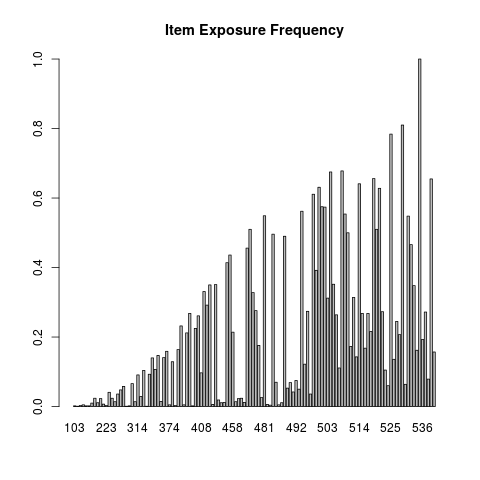
\includegraphics[scale = .45]{ItemExposureMFI.png}
  \end{center}
\end{frame}

\begin{frame}{New Method}
  \begin{center}
    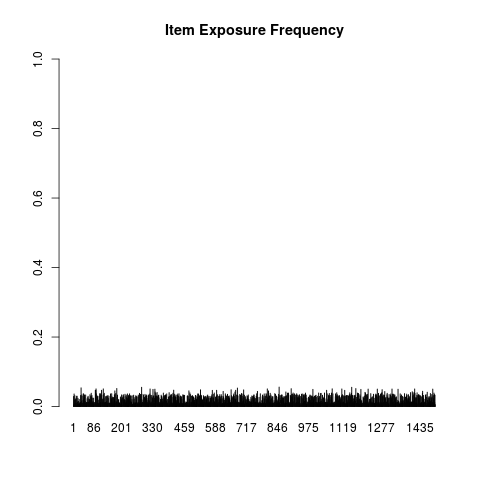
\includegraphics[scale = .45]{ItemExposure.png}
  \end{center}
\end{frame}

\begin{frame}{FSH}
  \begin{center}
    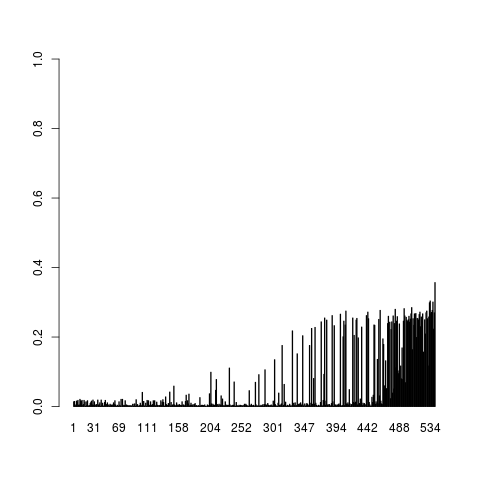
\includegraphics[scale = .45]{ItemExposureFSH.png}
  \end{center}
\end{frame}

\begin{frame}{AS-BB}
  \begin{center}
    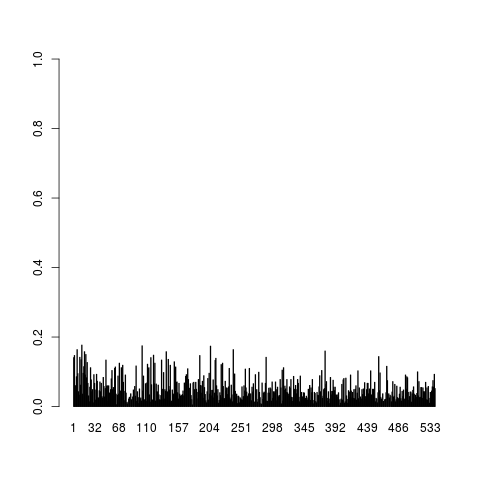
\includegraphics[scale = .45]{ItemExposureASBB.png}
  \end{center}
\end{frame}



\section{Discussion}
\begin{frame}{Limitations}
\begin{itemize}
\item Limitations:
  \begin{enumerate}[1)]
  \item Computationally intensive
  \item Tricky to specify apporpriatly
  \end{enumerate}
\end{itemize}
\end{frame}
   
\end{document}



%%% Local Variables:
%%% mode: latex
%%% TeX-master: t
%%% End:
